The first tool that we will make is a proof of concept GUI that allows an end user to interface with the functionality
we have created by interacting with a user interface that we create.

For the website we will be relying on the plotly tool~\cite{plotlydash} as it is a relatively simple tool that will
allow us to quickly reach a minimum viable product

Our end goal for such a GUI would be to expose every functionality that the discovery tool provides, presented as a neat
visualisation that requires very little understanding of the underlying logic.
Once this is achieved, we can look into building more complex functionality that relies on the discovery tool.

\subsection{data input}\label{subsec:data-input}
The first and simplest step we have is to read the data from somewhere.
To do this we will simply create a folder on the filesystem that will be read from, we can then set up a dash callback
to periodically check if there have been updates to the folder, which will allow us to inject files from any source.

\begin{figure}[h]
    \centering
    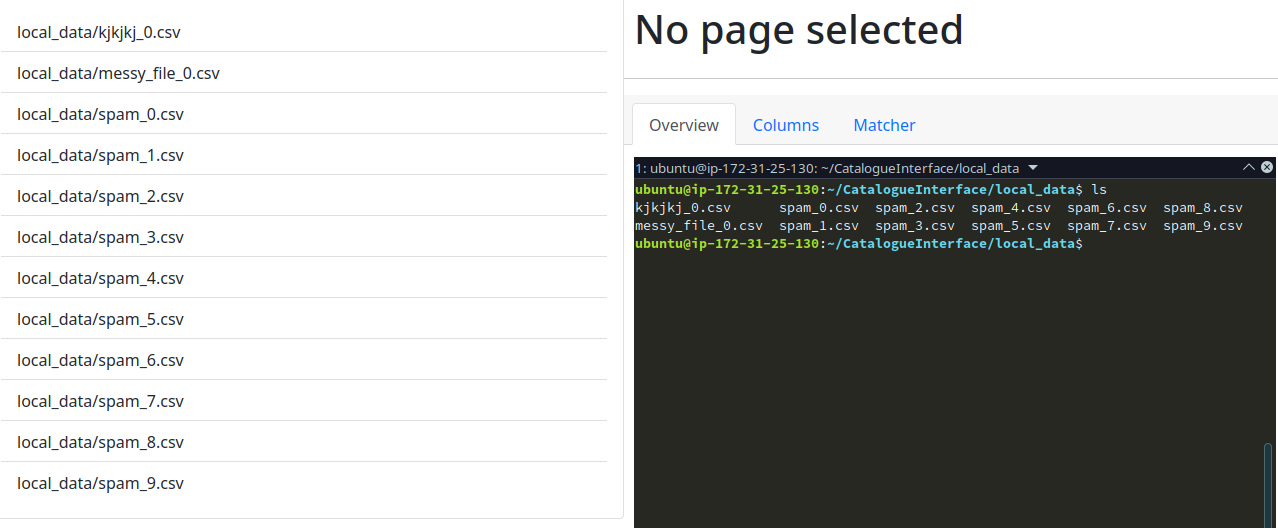
\includegraphics[width=12cm]{figures/website_images/website_data_catalogue}
    \caption{Demonstrating that the files in the data folder are being read}\label{fig:catalogue_file_list}
\end{figure}

Next, we need to implement a system to load from metadata, this will ensure that edits to metadata will stay permanent
when done from the UI\@.
TODO

\subsection{displaying metadata}\label{subsec:displaying-metadata}
When choosing a data file to look at, we would like to start by providing an overview of the file, giving surface level
information that a user can use to understand what they are looking at.
In our case we have chosen the pertinent information to be as follows:

- A list of tags assigned to the data file

- The file size and dimensions

- A snippet of the data file (such as displaying the first 10 rows)

- The ability to download the data file

\begin{figure}[h]
    \centering
    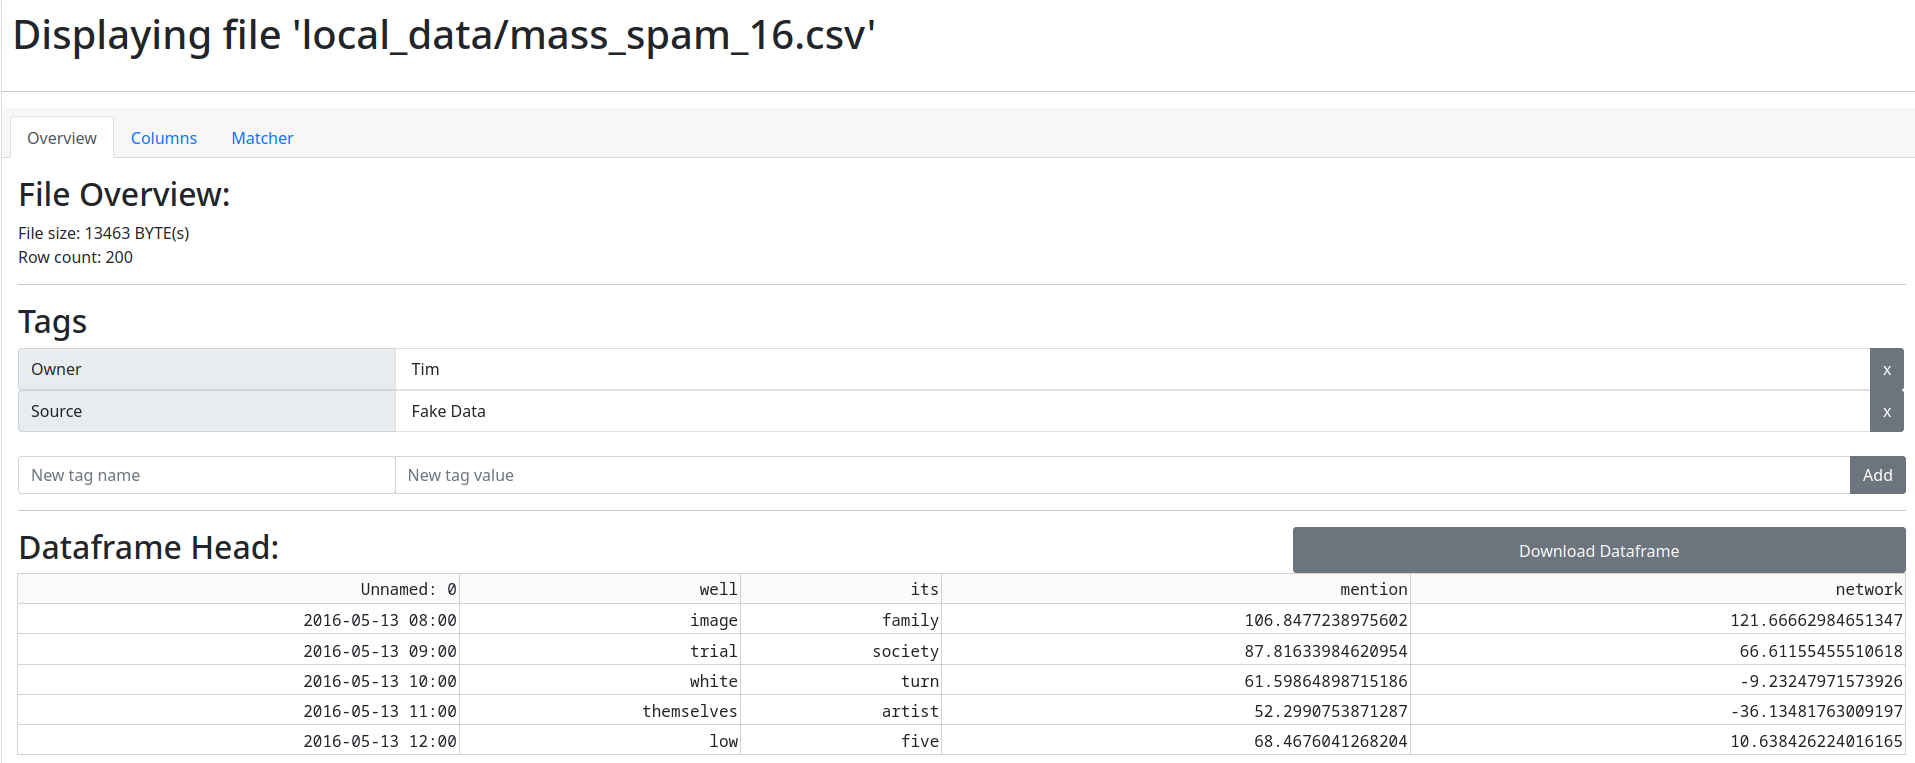
\includegraphics[width=12cm]{figures/website_images/catalogue_page_file_overview}
    \caption{Displaying an overview of the selected file}\label{fig:catalogue_file_overview}
\end{figure}

Our implementation, as pictured in ~\ref{fig:catalogue_file_overview} also includes the ability to add and remove
metadata tags.

\subsection{data generation}\label{subsec:data-generation}
